\PassOptionsToPackage{unicode=true}{hyperref} % options for packages loaded elsewhere
\PassOptionsToPackage{hyphens}{url}
%
\documentclass[ignorenonframetext,]{beamer}
\usepackage{pgfpages}
\setbeamertemplate{caption}[numbered]
\setbeamertemplate{caption label separator}{: }
\setbeamercolor{caption name}{fg=normal text.fg}
\beamertemplatenavigationsymbolsempty
% Prevent slide breaks in the middle of a paragraph:
\widowpenalties 1 10000
\raggedbottom
\setbeamertemplate{part page}{
\centering
\begin{beamercolorbox}[sep=16pt,center]{part title}
  \usebeamerfont{part title}\insertpart\par
\end{beamercolorbox}
}
\setbeamertemplate{section page}{
\centering
\begin{beamercolorbox}[sep=12pt,center]{part title}
  \usebeamerfont{section title}\insertsection\par
\end{beamercolorbox}
}
\setbeamertemplate{subsection page}{
\centering
\begin{beamercolorbox}[sep=8pt,center]{part title}
  \usebeamerfont{subsection title}\insertsubsection\par
\end{beamercolorbox}
}
\AtBeginPart{
  \frame{\partpage}
}
\AtBeginSection{
  \ifbibliography
  \else
    \frame{\sectionpage}
  \fi
}
\AtBeginSubsection{
  \frame{\subsectionpage}
}
\usepackage{lmodern}
\usepackage{amssymb,amsmath}
\usepackage{ifxetex,ifluatex}
\usepackage{fixltx2e} % provides \textsubscript
\ifnum 0\ifxetex 1\fi\ifluatex 1\fi=0 % if pdftex
  \usepackage[T1]{fontenc}
  \usepackage[utf8]{inputenc}
  \usepackage{textcomp} % provides euro and other symbols
\else % if luatex or xelatex
  \usepackage{unicode-math}
  \defaultfontfeatures{Ligatures=TeX,Scale=MatchLowercase}
\fi
% use upquote if available, for straight quotes in verbatim environments
\IfFileExists{upquote.sty}{\usepackage{upquote}}{}
% use microtype if available
\IfFileExists{microtype.sty}{%
\usepackage[]{microtype}
\UseMicrotypeSet[protrusion]{basicmath} % disable protrusion for tt fonts
}{}
\IfFileExists{parskip.sty}{%
\usepackage{parskip}
}{% else
\setlength{\parindent}{0pt}
\setlength{\parskip}{6pt plus 2pt minus 1pt}
}
\usepackage{hyperref}
\hypersetup{
            pdftitle={Git for Non-Programmers},
            pdfborder={0 0 0},
            breaklinks=true}
\urlstyle{same}  % don't use monospace font for urls
\newif\ifbibliography
\setlength{\emergencystretch}{3em}  % prevent overfull lines
\providecommand{\tightlist}{%
  \setlength{\itemsep}{0pt}\setlength{\parskip}{0pt}}
\setcounter{secnumdepth}{0}

% set default figure placement to htbp
\makeatletter
\def\fps@figure{htbp}
\makeatother


\title{Git for Non-Programmers}
\author{Fernando Hoces de la Guardia\\
BITSS\\
-\\
Slides at\\
\hspace*{0.333em}\url{https://github.com/BITSS/CEGA2019}}
\date{CEGA, October 2019}

\begin{document}
\frame{\titlepage}

\begin{frame}
\tableofcontents[hideallsubsections]
\end{frame}
\hypertarget{reproducible-workflow}{%
\section{Reproducible Workflow}\label{reproducible-workflow}}

\begin{frame}{The Claerbout Principle}
\protect\hypertarget{the-claerbout-principle}{}

\begin{quote}
An article about computational science in a scientific publication is
not the scholarship itself, it is merely advertising of the scholarship.
The actual scholarship is the complete software development environment
and the complete set of instructions which generated the figures.
\end{quote}

\href{https://statweb.stanford.edu/~wavelab/Wavelab_850/wavelab.pdf}{Buckheit
\& Donoho, 1995}

\end{frame}

\begin{frame}{Organizing Principles}
\protect\hypertarget{organizing-principles}{}

Christensen, Miguel \& Freese (2019)

1 - Use code (scripts), don't work by hand (Excel/spreadsheet).\\
2 - Consider not saving statistical output, and just saving the code and
raw data that generates it.\\
3 - Reproducibility--on your own machine across multiple runs, across
machines, across researchers.

\end{frame}

\begin{frame}{File Management \& Coding Suggestions}
\protect\hypertarget{file-management-coding-suggestions}{}

Begin with a logical file structure
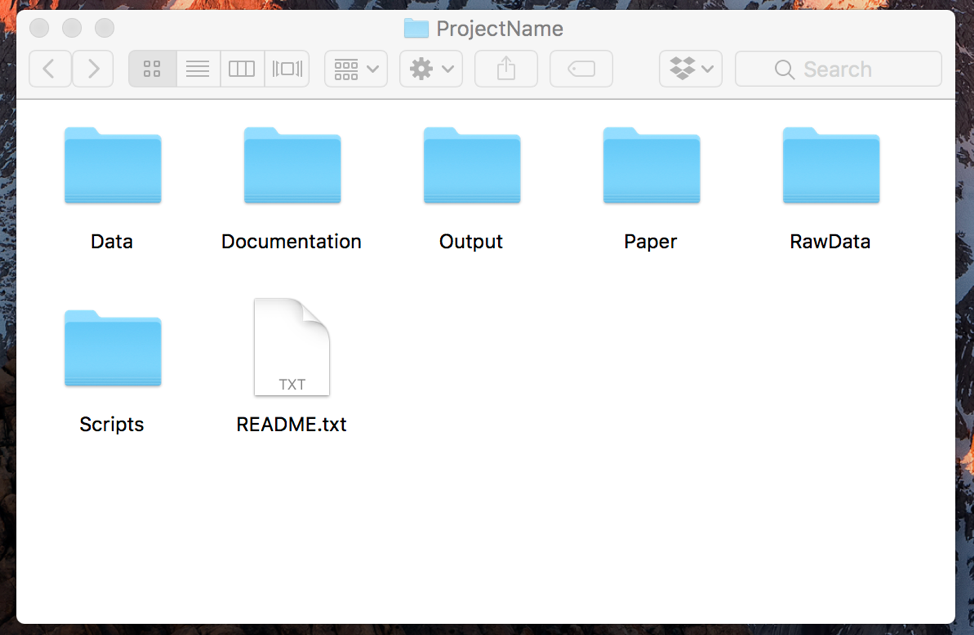
\includegraphics[height=2.25in]{../Images/files.png}

\end{frame}

\hypertarget{version-control}{%
\section{Version Control}\label{version-control}}

\begin{frame}{Git/Github for Version Control}
\protect\hypertarget{gitgithub-for-version-control}{}

\begin{itemize}
\item
  Git and Github are tools to track the complete history of your files.
\item
  They are very popular among programmers, but not so much among
  non-programmers.
\item
  Why? I believe it has to do with GUIs.
\end{itemize}

\end{frame}

\begin{frame}{What is a GUI and why the bad reputation}
\protect\hypertarget{what-is-a-gui-and-why-the-bad-reputation}{}

\textbf{G}raphical \textbf{U}ser \textbf{I}nterface

\begin{itemize}
\item
  For most of us (non-programmers): \(GUI = Software\).
\item
  GUIs are behind the popularization of personal computers.
\item
  Unfortunately GUIs are pretty bad at keeping a record of actions taken
  (bad for reproducibility).
\end{itemize}

\end{frame}

\begin{frame}{What is not a GUI?}
\protect\hypertarget{what-is-not-a-gui}{}

\begin{itemize}
\tightlist
\item
  Any software that is run in the command line (aka terminal, shell,
  bash, etc).
\end{itemize}

\centering

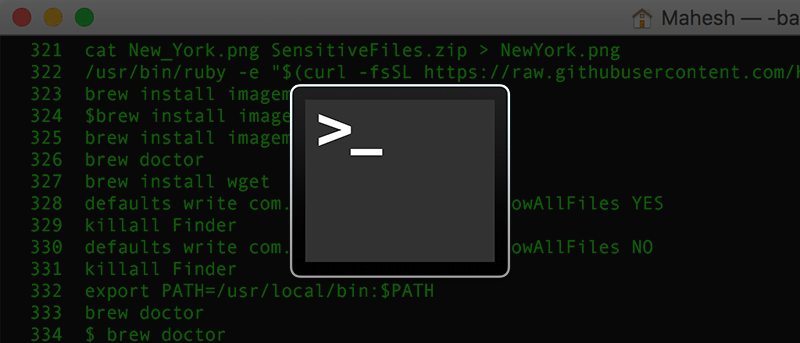
\includegraphics[height=1in]{../Images/command_line.png}

\begin{itemize}
\item
  Git was designed to run in the command line.
\item
  Today we will learn Git \textbf{without} the command line.
\end{itemize}

\end{frame}

\begin{frame}{What is Git 1/2}
\protect\hypertarget{what-is-git-12}{}

\begin{itemize}
\item
  Git is a software designed to track the \textbf{entire} history of the
  code of a project.
\item
  Designed originally for software development, it has gained important
  traction in the research community.
\item
  Main appeal: facilitates full reproducibility and collaboration.
\item
  Git is mainly meant to work as a non-GUI (in the command line)
  software.\\
  \textbf{However:} most of the key features can be used through a GUI.
\end{itemize}

\end{frame}

\begin{frame}[fragile]{What is Git 2/2}
\protect\hypertarget{what-is-git-22}{}

\begin{itemize}
\item
  By code git understands any type of plain text file
  (\texttt{myfile.R}, \texttt{myfile.do},
  \texttt{.tex/.md/.txt/.csv/.etc}).
\item
  This types of files can be understood as ``human readable'' as machine
  and human see the same fie.
\item
  Files that are ``non-human readable'' are called binary files
  (\texttt{myfile.docx}, \texttt{myfile.xlxs},
  \texttt{.pdf/.exe/.dta/.etc}).
\item
  Git can also detect changes in binary files, but it cannot show those
  changes.
\end{itemize}

\end{frame}

\begin{frame}{What is Github}
\protect\hypertarget{what-is-github}{}

\begin{itemize}
\item
  Github is a company that provides two services (that we care of):

  \begin{itemize}
  \tightlist
  \item
    A web hosting service for all our files track with git (public
    free/private \$ or free if academic).\\
  \item
    A GUI software (Desktop App) that provides user friendly access to
    git.
  \end{itemize}
\item
  Others hosting ss include: Bitbucket, GitLab, Gitkraken, etc.
\item
  Other GUIs include: SourceTree, Gitkraken, Atom, RStudio.
\end{itemize}

\end{frame}

\begin{frame}{The Primary Goal of Version Control (for us)}
\protect\hypertarget{the-primary-goal-of-version-control-for-us}{}

\textbf{The Goal:} keep track of any potentially meaningful modification
to your code.\\
\pause   \textbf{Secondary Goal:} Learn how to collaborate with others
using Github.

\pause

\textbf{Bonus track:} get you excited about using open source
statistical software (R, Python, Julia, etc)

\end{frame}

\begin{frame}[fragile]{Strategy 1:}
\protect\hypertarget{strategy-1}{}

1 - Agree on a naming convention with you co-authors (eg:
YYYYMMDDfilename\_INITALS).\\
2 - Begin working from the last saved version (eg:
\texttt{20180325demo\_FH.do}).\\
3 - At the end of the day, save on a new version (eg:
\texttt{20180327demo\_FH.do}).

\textbf{Pros:} Easy adoption.

\textbf{Cons:} Error prone, hard to document, lots of files for each
document.

\end{frame}

\begin{frame}[fragile]{Strategy 2:}
\protect\hypertarget{strategy-2}{}

1 - Name your file \texttt{filename} (ideally \texttt{01\_filename})\\
2 - Take a snapshot of your work every time you complete relevant change
(day, hour or minutes).\\
3 - Update your entire working folder to the cloud.

\textbf{Pros:} Error proof, seamless documentation, one file per
document, track differences across all versions, meant to work with the
cloud.

\textbf{Cons:} Harder adoption.

\end{frame}

\begin{frame}{We want to avoid this situation:}
\protect\hypertarget{we-want-to-avoid-this-situation}{}

\centering


\includegraphics[height=2.8in]{../Images/phdcomics.png}

\end{frame}

\begin{frame}{Comparison of Workflows}
\protect\hypertarget{comparison-of-workflows}{}

\hspace*{-0.35in}{
\includegraphics[height=2.8in]{../Images/version_control_diagram.png}}

\end{frame}

\begin{frame}{Other reasons to use git}
\protect\hypertarget{other-reasons-to-use-git}{}

\begin{itemize}
\tightlist
\item
  To access a whole new world of knowledge!\\
\item
  Great tool for collaboration.\\
\item
  Easier to test all sorts of ideas/models.
\end{itemize}

\end{frame}

\begin{frame}{Managing expectations}
\protect\hypertarget{managing-expectations}{}

\centering

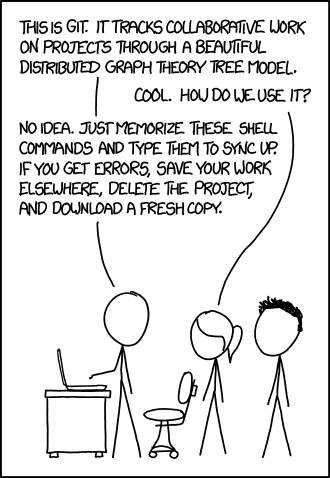
\includegraphics[height=3in]{../Images/git.png}

\end{frame}

\hypertarget{demos}{%
\section{Demos}\label{demos}}

\begin{frame}{Five Demos:}
\protect\hypertarget{five-demos}{}

1 - \textbf{Simple but instructive.}

2 - Repeat with branches.

3 - Repeat with collaboration: pull requests.

4 - Repeat with collaboration: shared ownership.

5 - Explore a real life repo.

\end{frame}

\begin{frame}{Demo \#1: We Start in the Cloud}
\protect\hypertarget{demo-1-we-start-in-the-cloud}{}

1 - Create \url{github.com} account and sign in.\\
2 - Let's look at some \textbf{repos}.\\
3 - First way to access content: download.\\
4 - What if you want to have your own copy of the repo? \textbf{Fork}
it!.\\
5 - Now create your own repo. Initiate readme and make some edits.

\end{frame}

\begin{frame}{Demo \#1: We move to our local computer}
\protect\hypertarget{demo-1-we-move-to-our-local-computer}{}

6 - Clone the it. Explore the files and location.\\
7 - Create new files, edit. And commit. Edit again, and commit again.\\
8 - Push. Edit on github.com, and pull.\\
9 - For this tutorial, best way to access previous version: explore in
github.com and download.

\end{frame}

\begin{frame}{Five Demos 2/5:}
\protect\hypertarget{five-demos-25}{}

1 - Simple but instructive.\\
\emph{Review: def repo, github.com, download, clone, destination folder,
fork, create repo, commit, push, pull, delete, search repo, download old
version.}

2 - \textbf{Repeat with branches.}

3 - Repeat with collaboration: pull requests.

4 - Repeat with collaboration: shared ownership.

5 - Explore a real life repo.

\end{frame}

\begin{frame}{Demo \#2: Branches and collaboration (we wil be here a
while)}
\protect\hypertarget{demo-2-branches-and-collaboration-we-wil-be-here-a-while}{}

1 - Create a branch from previous repo.\\
2 - Add new content (do not replace), commit a few times, and go back
and forth to the main branch.\\
3 - Go back to main branch (master), observe file, merge.\\
4 - Look at the history of the main branch.\\
5 - Repeat 1-3 but now replace instead of adding content.

\end{frame}

\begin{frame}{Fatal Error!}
\protect\hypertarget{fatal-error}{}

\centering

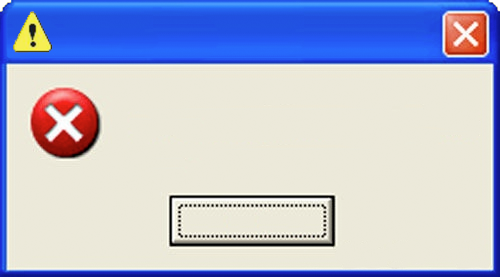
\includegraphics[height=1in]{../Images/error_image.png}

\pause


\includegraphics[height=1.8in]{../Images/calm_burn.jpg}

\LARGE{Burn it and start with a fresh copy!}

\end{frame}

\begin{frame}{Five Demos: 3/5}
\protect\hypertarget{five-demos-35}{}

1 - Simple but instructive.\\
Review: def repo, github.com, download, clone, destination folder, fork,
create repo, commit, push, pull, delete, search repo, download old
version.\\
2 - Repeat with branches.\\
\emph{Review: All of the above, plus: branch, merge, resolve
conflicts.}\\
3 - \textbf{Repeat with collaboration: pull requests.}\\
4 - Repeat with collaboration: shared ownership.\\
5 - Explore a real life repo.

\end{frame}

\begin{frame}{Demo \#3: Pull requests}
\protect\hypertarget{demo-3-pull-requests}{}

1 - Fork repo
\href{https://github.com/BITSS/test_birthday}{github.com/BITSS/test\_birthday},
and clone it into your machine.\\
2 - Edit fields of name, and birth date.\\
3 - Save, commit and push.\\
4 - Create your first \textbf{pull request}.\\
5 - Let's see if I can manage all those pull requests very quickly
(maybe illustrate issues).\\
6 - Now find your neighbors repo of Demos 1 \& 2, fork it, clone it,
make a change, save, commit, and\ldots{}

\end{frame}

\begin{frame}{Two formats of collaboration}
\protect\hypertarget{two-formats-of-collaboration}{}

\begin{itemize}
\tightlist
\item
  One owner, many pull requests.

  \begin{itemize}
  \tightlist
  \item
    Easier to control, requires constant updating.\\
  \end{itemize}
\item
  Many owners, all can push.

  \begin{itemize}
  \tightlist
  \item
    \textbf{Very} important to pull at the beginning and at before each
    push.
  \end{itemize}
\end{itemize}

\end{frame}

\begin{frame}{Five Demos: 4/5}
\protect\hypertarget{five-demos-45}{}

1 - Simple but instructive.\\
Review: def repo, github.com, download, clone, destination folder, fork,
create repo, commit, push, pull, delete, search repo, download old
version.\\
2 - Repeat with branches.\\
Review: All of the above, plus: branch, merge, resolve conflicts.\\
3 - Repeat with collaboration: pull requests.\\
\emph{Review: collaborate via fork + PR}\\
4 - \textbf{Repeat with collaboration: shared ownership. }\\
5 - Explore a real life repo.

\end{frame}

\begin{frame}{Demo \#4: Many owners}
\protect\hypertarget{demo-4-many-owners}{}

1 - Half of you (\#1): go back to the repo of demo 1 \& 2 and invite a
collaborator.\\
(Suggestion: the ``forker'' creates the repo, the ``forkee'' is
invited\\
, edit, commit, push/pull)\\
\pause   2 - The other half (\#2): clones, commits and pushes.\\
\pause   3 - \#1 commits and pushes in \textbf{different lines}.\\
\pause   4 - Switch and repeat 2 \& 3: \#2 commits first and pushes,
then \#1.\\
\pause   5 - Repeat 2 - 4 but now both of you in the same lines.\\
\pause   6 - Repeat now but with branches (optional).

\end{frame}

\begin{frame}{Five Demos: 4/5}
\protect\hypertarget{five-demos-45-1}{}

1 - Simple but instructive.\\
Review: def repo, github.com, download, clone, destination folder, fork,
create repo, commit, push, pull, delete, search repo, download old
version.\\
2 - Repeat with branches.\\
Review: All of the above, plus: branch, merge, resolve conflicts.\\
3 - Repeat with collaboration: pull requests.\\
Review: collaborate via fork + PR\\
4 - Repeat with collaboration: shared ownership.\\
\emph{Review: collaborate via share ownership.}\\
5 - \textbf{Explore a real life repo. }

\end{frame}

\begin{frame}[fragile]{Demo \#5: Look inside a real-life project (and
collaborate!)}
\protect\hypertarget{demo-5-look-inside-a-real-life-project-and-collaborate}{}

1- Find the following repo: \texttt{github.com/BITSS/opa-wealthtax}.\\
2- Fork it and clone it.\\
3- Open it in your computer: \texttt{opa-wealthtax.Rproj} (needs
RStudio), look around and execute
\texttt{code/dynamic\_doc/wealth\_tax\_dd.Rmd}.\\
4- Find elasticities, fill in csv, document, submit. 5 - Find
\texttt{code/interactive\_visualization/server.R} and in line
\texttt{1561} change \texttt{red} to \texttt{blue}

\end{frame}

\begin{frame}{Five Demos: 5/5}
\protect\hypertarget{five-demos-55}{}

1 - Simple but instructive.\\
Review: def repo, github.com, download, clone, destination folder, fork,
create repo, commit, push, pull, delete, search repo, download old
version.\\
2 - Repeat with branches.\\
Review: All of the above, plus: branch, merge, resolve conflicts.\\
3 - Repeat with collaboration: pull requests.\\
Review: collaborate via fork + PR\\
4 - Repeat with collaboration: shared ownership.\\
Review: collaborate via share ownership.\\
5 - Explore a real life repo.\\
\emph{Review: All of the above, plus: how does a real-life example looks
like.}

\end{frame}

\begin{frame}{Bonus Demo: Look inside a half-way project (and
collaborate!)}
\protect\hypertarget{bonus-demo-look-inside-a-half-way-project-and-collaborate}{}

Description:

\begin{itemize}
\item
  Half baked project, forgotten from a few years.\\
\item
  Exploratory analysis of publication trends in NBER working paper
  series. Back then inspired by a paper from
  \href{https://eml.berkeley.edu/~sdellavi/wp/CardDellaVignaTop5PapersJEL2013.pdf}{DellaVigna
  and Card}.\\
\item
  Now there is more literature around this:
  \href{http://www.nber.org/papers/w23953}{Chari and Goldsmith-Pinkham}.
\item
  I will use github to share my work with you, do a little exercise, and
  invite you to collaborate.
\end{itemize}

\end{frame}

\begin{frame}[fragile]{Demo \#X: Look inside a half-way project (and
collaborate!)}
\protect\hypertarget{demo-x-look-inside-a-half-way-project-and-collaborate}{}

1- Find the following repo: \texttt{github.com/fhoces/nber\_trends}.\\
2- Fork it and clone it.\\
3- Open it in your computer: \texttt{nber\_trends.Rproj} (needs
RStudio), look around and execute up to the section
(\texttt{Verifying\ gender\ {[}WORKSHOP\ SECTION{]}}).\\
4- Generate random number like this:
\texttt{num1\ =\ sample(20000,\ 1)}.\\
5- Look the name and (imputed) gender of the author in row
\texttt{num1}. This is done by typing:\\
\texttt{temp3{[}num1,c("name",\ "gender"){]}} in the console.\\
6- Create the following line at the end of the script:
\texttt{verification\ \textless{}-\ cbind(temp3{[}num1,c("name",\ "gender"){]},\ "rownum"\ =\ num1,\ "correct"\ =\ 1)}.\\
7- Save, commit, push and create a pull request.\\
8- Feel free to look around create more contributions if you like. Happy
to co-author.

\end{frame}

\begin{frame}{Now go and explore!}
\protect\hypertarget{now-go-and-explore}{}

Some good habits:\\
- Commit often (\textless{}1hr)\\
- Always pull before you start a new session of work. Also good to pull
before pushing.\\
- Think of your remote as the most important set of files. Get used to
deleting things in your local machine.

\end{frame}

\begin{frame}{Want to learn more:}
\protect\hypertarget{want-to-learn-more}{}

\begin{itemize}
\item
  \href{https://www.youtube.com/watch?v=eWxxfttcMts}{Great 20 min intro
  to Git by Alice Bartlett}
\item
  \href{https://www.rstudio.com/resources/videos/happy-git-and-gihub-for-the-user-tutorial/}{Great
  2hr tutorial to Github by Jenny Bryan (git ninja)}
\item
  Jenny Bryan's \href{http://happygitwithr.com/}{Happy Git};
  \href{http://web.stanford.edu/~gentzkow/research/CodeAndData.pdf}{Documentation
  from Matthew Gentzkow and Jesse Shapiro}; Karthik Ram's paper on
  \href{https://scfbm.biomedcentral.com/articles/10.1186/1751-0473-8-7}{Git
  for Research}
\item
  Software Carpentry's
  \href{https://swcarpentry.github.io/git-novice/}{step-by-step tutorial
  (command line)}.
\end{itemize}

\end{frame}

\end{document}
